\documentclass[cap,cs5size,nospace,indent,fancyhdr]{ctexart}
\usepackage{booktabs}
\usepackage{caption}  
\usepackage{changepage}
\usepackage{geometry}
 \usepackage{pgfplots}
 \usepgfplotslibrary{dateplot}
\geometry{top=2cm,bottom=2cm}
\usepackage{tcolorbox}
\usepackage{xpinyin}
\usepackage{subfigure}
\usepackage{float}
\usepackage{multicol}
\usepackage[T1]{fontenc}
\usepackage[utf8]{inputenc}
\usepackage{authblk}

\title{Math 286 Lab Project}
\date{2020, Sept, 11th}
\author{\textbf{Ruan Yucheng} 3180111}
\author{\textbf{Zhang Zheyuan} 3180111607}
\author{\textbf{Wu Zheyu} 3180111}
\author{\textbf{Qian Chen} 3180111591}
\author{\textbf{Zheng Xiuwen} 3180111}
\affil{Department of Mechanical Engineering, ZJUI}
\renewcommand\Authands{ and }

\begin{document}
\maketitle

\section{Problem 1}
Determine the maximal solution of the following ODE with the initial value.
\begin{equation}
	y' = t^2+y^3, y(0)=1
\end{equation}
\subsection{Direction Field}
At first, we plot the direction field of (1). After connecting the direction arrows we find that the curve seems has 2 vertical asymptotes, which approximately lies between -2.1 to -2.2 and 0.8 to 0.9.

\begin{center}
	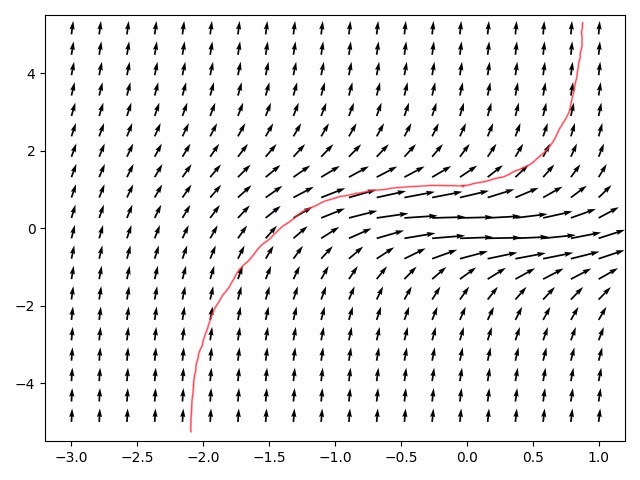
\includegraphics[scale=0.3]{HandSketch.jpeg}
\end{center}

\subsection{Numerical Methods}

\subsubsection{Methods}
\begin{multicols}{2}	
	\textbf{Euler}: <code>
	
	$ y_{n+1} = y_n+h*f(t_n, y_n)$
	
	$ t_{n+1} = t_n+h$
	
	\vfill\null
	\columnbreak

	\textbf{Heun}: <code>
	
	$ k_{1,n} = f(t_n,y_n)$
	
	$ k_{2,n} = f(t_n+h, y_n+h*k_{1,n})$
	
	$ y_{n+1} = y_n+h*f(t_n, y_n)$
	
	$ t_{n+1} = t_n+h$
	

	\textbf{Runge Kutta}: <code>
	
	$ k_{1,n} = f(t_n,y_n)$
	
	$ k_{2,n} = f(t_n+\frac{h}{2}, y_n+\frac{h}{2}*k_{1,n})$

	$ k_{3,n} = f(t_n+\frac{h}{2}, y_n+\frac{h}{2}*k_{2,n})$

	~\\

	$ k_{4,n} = f(t_n+h, y_n+h*k_{3,n})$
	
	$ y_{n+1} = y_n+\frac{h}{6}*(k_{1,n}+2*(k_{2,n}+k_{3,n})+k_{4,n})$
	
	$ t_{n+1} = t_n+h$

	\vfill\null
	\columnbreak
\end{multicols}

\subsubsection{Rough Approximation}
\noindent First we apply three methods all together with a step of $h = 0.1$ obtain the table below:
\begin{table}[!htb]
	\begin{center}
		\begin{tabular}{l|r|r|r|r|r|r|r|r}
			\textbf{T} & \textbf{-2.3} & \textbf{-2.2} &\textbf{-2.1} & \textbf{-2.0} & \textbf{0.7} & \textbf{0.8} & \textbf{0.9} & \textbf{1.0}  \\
			\hline
			Euler & -19.87 & -9.10 & -5.05 & -3.08 & 3.41 & 4.85 & 7.66 & 14.31\\	
			\hline
			Heun  &-5.48E5&-175.74&-17.44 & -6.25 & 5.36 & 11.14 & 48.95 & 4479.18\\
			\hline
			RK & -1.62E99 & -2.59E7 & -36.57 & -7.12 & 5.89 & 16.04 & 2777.84 & 5.43E35\\
		\end{tabular}
	\end{center}
\end{table}

Combined with the table, the direction field and the hand-drawing sketches, we could find that the results diverses dramatically large around -2.2 to -2.1 and 0.8 to 0.9. Therefore, our next step is 
\end{document}